\section{Theorie}
\label{sec:Theorie}


\subsection{Der LC-Kreis}
Der $LC$-Kreis gehört zu den ungedämpften Schwingkreisen.Unter diesen wird
 ein System mit zwei Energiespeichern, zwischen denen eine vorher eingeführte Energiemenge
  oszilliert, verstanden. Bei einem $LC$-Kreis sind die Speicher durch eine Kapazität $C$ sowie
  eine Induktivität $L$ realisiert. Da im theoretischen $LC$-Kreis kein Bauteil mit Energieverbrauch
   existiert, bleiben Oszillation und Anfangsamplitude zeitlich erhalten.

   \begin{figure}[H]
     \centering
     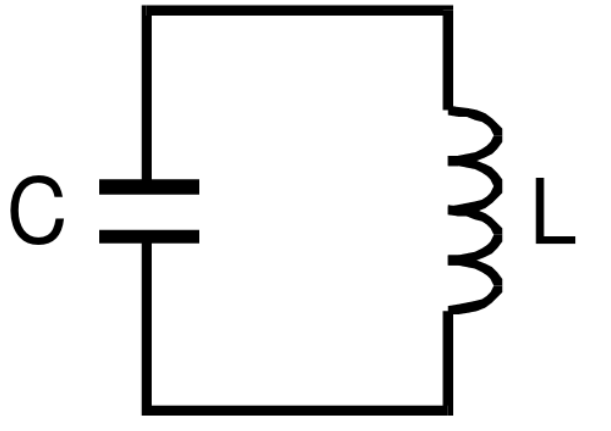
\includegraphics[width=\linewidth-300pt,height=\textheight-300pt,keepaspectratio]{content/CL.png}
     \caption{Schaltskizze eines $LC$-Kreises \cite{V354}.}
     \label{fig:CL_Kreis}
   \end{figure}

   \subsection{Der RCL-Kreis}
Eine Erweiterung des Systems ist der $RCL$-Kreis, in dem eine gewisse Energierate
kontinuierlich über einen ohmschen Widerstand $R$ in Wärme umgesetzt wird. Als Folge sind
die Kondensatorspannung $U_C(t)$ und die Stromstärke $I(t)$  monoton fallende Funktionen der Zeit. Es handelt sich daher um eine gedämpfte
 Schwingung.
 \begin{figure}[H]
   \centering
   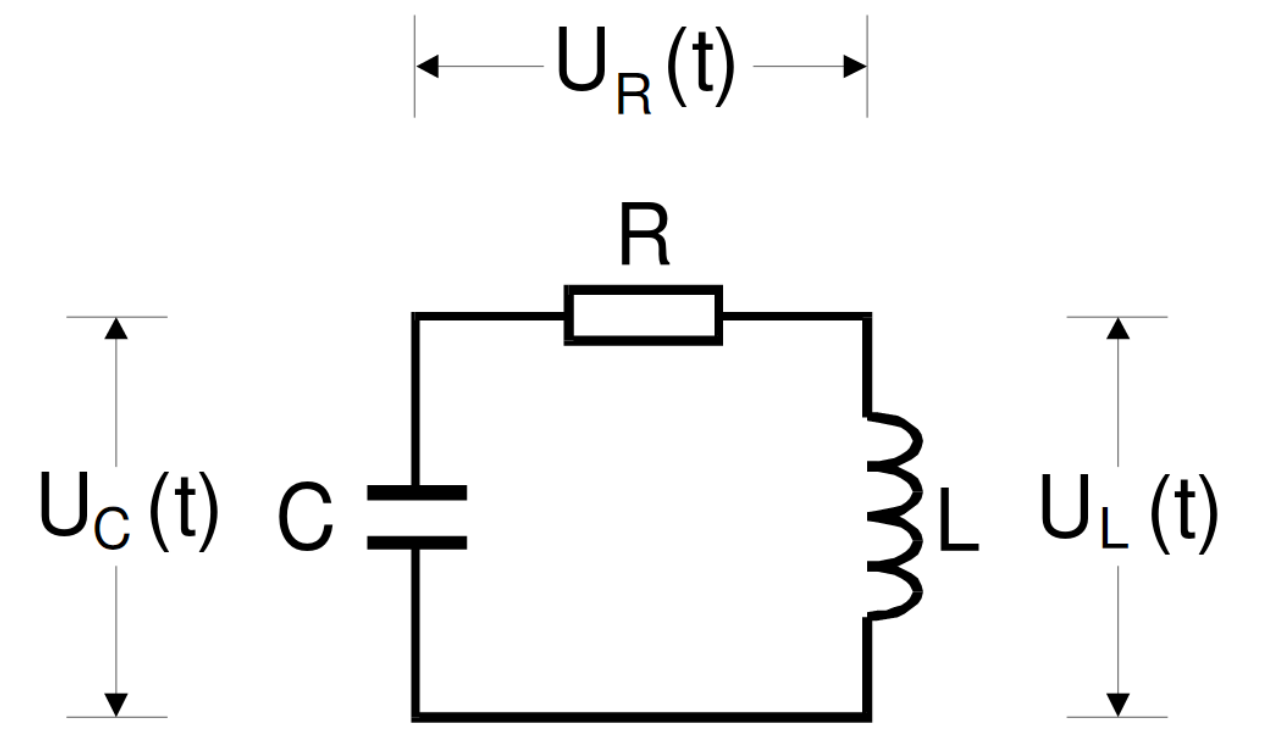
\includegraphics[width=\linewidth-200pt,height=\textheight-200pt,keepaspectratio]{content/RCL.png}
   \caption{Schaltskizze eines $RCL$-Kreises \cite{V354}.}
   \label{fig:RCL_Kreis}
 \end{figure}
Nach den kirchhoffschen Regeln folgt die DGL:
 \begin{equation}
   \ddot{I} + \frac{R}{L} \dot{I} + \frac{1}{LC}I = 0\text{.}
 \end{equation}
 Mit einem komplexen $e$-Ansatz erhält man die Konstanten $k_{1,2}$ der Zielfunktion.
 \begin{equation}
   \overline{k_{1,2}} = \frac{R}{2L}i \pm \sqrt{\frac{1}{LC}-\frac{R²}{4L²}}\text{.}
 \end{equation}
 Diese lassen sich aufteilen:
 Der Parameter $\mu$ beschreibt die Dämpfungskonstante des Systems:
 \begin{equation}
 \mu = \frac{R}{2L}
 \end{equation}
 Die Winkelgeschwindigkeit $\omega_0$ bezeichnet die Winkelgeschwindigkeit des Systems, läge keine Dämpfung vor:
 \begin{equation}
 w_0 = \sqrt{\frac{1}{LC}}
 \end{equation}
 Die Winkelgeschwindigkeit $\omega_{res}$ bezeichnet hingegen die Winkelgeschwindigkeit des gedämpften Systems:
 \begin{equation}
 w_{\text{res}} = \sqrt{w_0^2-\mu^2}
 \end{equation}
  Daher ergibt sich:
 \begin{equation}
	 \overline{k_{1,2}} = \mu i \pm w_{res}\text{.}
 \end{equation}
 Hiermit gelangt man zur allgemeinen Lösung:
 \begin{equation}
   I(t) = e^{-\mu t} \cdot  \operatorname{Re}\left( A_1e^{i\omega_{res} t} + A_2e^{-i\omega_{res} t} \right) \text{ mit } A_1\text{, } A_2 \text{ komplex.}
 \end{equation}
 Die endgültige Form der Lösungsfunktion hängt nun vom Aussehen von $\omega_res$ ab.
  Es wird zwischen 3 Fällen unterschieden.
  \begin{itemize}

  \item Gilt $\omega_0 > \mu $, wird die Lösungsfunktion nach (7) komplex und es liegt eine gedämpfte Schwingung vor.
  In diesem Fall lässt sich $I(t)$ durch
  \begin{equation}
    I(t) = A_0 e^{-\mu t} \cdot cos(\omega_{res} t + \varphi)
  \end{equation}
  ausdrücken. Die Periodendauer des schwingenden Systems ist dann:
  \begin{equation}
    T = \frac{2 \pi}{\omega_{res}}\text{.}
  \end{equation}
  Für die Ablinkdauer $\tau$ der Amplituden folgt zudem aus (3):
  \begin{equation}
    \tau = \frac{2L}{R}\text{.}
  \end{equation}

  \item Liegt $\omega_0 < \mu $ vor wird die Lösungsfunktion nach (7) reell und es liegt eine Dämpfung vor. Diese zeigt nach hinreichender Zeit ein einfaches Relaxationsverhalten.
   Je nachdem wie die Parameter $A_1$ und $A_2$ bestimmt sind, kann $I(t)$ vorher jedoch noch einen
   Maximalwert durchlaufen.
   \begin{figure}[H]
     \centering
     \includegraphics[width=\linewidth-200pt,height=\textheight-200pt,keepaspectratio]{content/dämpfungen.png}
     \caption{Relaxationsverhalten bei verschiedenen aperiodischen Dämpfungen \cite{V354}.}
     \label{fig:Dämpfungen}
   \end{figure}

\item Ist $\omega_0 = \mu $ erfüllt, liegt der aperiodische Grenzfall vor. Bei diesem, in der Darstellung schwarz gestrichelt,
 durchläuft $I(t)$ kein Maximum und flacht am schnellsten ab.

\end{itemize}



\subsection{ Der RCL-Kreis unter Einfluss einer erzwungenen Schwingung}

Wenn ein gedämpfter Schwingkreis einer äußeren periodischen Kraft $F(t)$, im Fall des $RCL$-Kreises
 einer Wechselspannung der Winkelgeschwindigkeit $\omega$, unterworfen wird, zeigen sich einige Eigenschaften.
Für die DGL des Schwingkreises folgt dann:
\begin{equation}
  LC \ddot{U}_C + RC \dot{U}_C + U_C = U_{\text{Antrieb}} =A_{\text{Antrieb}} \cdot \operatorname{Re}\left( e^{i\omega t}\right)\text{.}
\end{equation}
Mithilfe eines komplexen $e$-Ansatzes für $U_C$ erhält man für den Betrag der zugehörigen Amplitude $A_C$:
\begin{equation}
  A_C(\omega) = \frac{A_{\text{Antrieb}}}{\sqrt{(1-LC\omega^2)^2 + \omega^2R^2C^2}}\text{.}
\end{equation}
Es zeigt sich beim angetriebenen $RCL$-Kreis eine Phasenverschiebung $\varphi$ zwischen $U_C$ und $U_{\text{Antrieb}}$.
Für diese gilt:
\begin{equation}
  \varphi(\omega) = \arctan\left( \frac{-\omega RC}{1-LC \omega^2}\right)\text{.}
\end{equation}
Es zeigt sich, dass $U_C$ und $U_{\text{Antrieb}}$ für hinreichend kleine Frequenzen weiterhin in Phase sind,
während $U_C$ für sehr hohe Frequenzen $\varphi \approx \frac{\pi}{2}$ hinter $U_{\text{Antrieb}}$ zurückbleibt.



\subsection{Resonanzen und Güte eines angetriebenen RCL-Kreises}

Die Amplitude der Kondensatorspannung ist daher abhängig von der Frequenz der Generatorspannung.
Für $\omega \to \infty$ läuft $U_C$ gegen 0, für $\omega \to 0$ gegen $A_{\text{Antrieb}}$.
Für eine Frequenz $f_{res}$ erreicht $U_C$  jedoch ein Maximum, welches größer als $A_{\text{Antrieb}}$ selbst ist.
Diese Frequenz wird als Resonanzfrequenz des Systems bezeichnet. Für $f_{res}$ gilt:
\begin{equation}
  f_{res} = \frac{\omega_{res}}{2\pi} = \frac{\sqrt{\frac{1}{LC}-\frac{R^2}{2L^2}}}{2 \pi}\text{.}
  %f_{res} = \frac{\sqrt{\frac{1}{LC} - \frac{R^2}{2L^2}}{2 \pi}}
\end{equation}
Bei auftretender Resonanz ist zwischen zwei Fällen zu unterscheiden.
In dem Fall einer schwachen Dämpfung, also $\frac{R^2}{2L^2} \ll \frac{1}{LC}$, wird  $A_{C,max}$ durch
\begin{equation}
  A_{C,max} = \frac{A_{\text{Antrieb}}}{\omega_0 RC}
  %A_{C,max} = \frac{U_0}{R} \cdot \sqrt{\frac{L}{C}}
\end{equation}
beschrieben.
 Läuft $R$ dann auch noch gegen 0, strebt $A_{C,max}$ gegen unendlich und es kommt zu einer
Resonanzkatastrophe.
 Der Faktor $\frac{1}{\omega_0 RC}$ wird auch als Güte $q$ bezeichnet.
Letztere lässt sich mit
\begin{equation}
  q = \frac{\sqrt{LC}}{RC}
  \end{equation}
bestimmen. Die Stellen links und rechts neben dem Maximum,
 an denen $A_C$ $\frac{1}{\sqrt{2}}$ von $A_{C,max}$ erreicht, werden als $\omega_-$ bzw. $\omega_+$ bezeichnet.
 Ist die Güte bekannt lassen sie sich über
 \begin{equation}
   \omega_{+,-} = \sqrt{-\frac{R²C²-2LC}{2L²C²} \pm \sqrt{\left( \frac{R²C²-2LC}{2L²C²} \right) ^2 - \frac{1- \frac{2}{q²}}{L²C²}}}
 \end{equation}
 ermitteln.
 Die Breite der Resonanzkurve wird durch
 \begin{equation}
   \omega_+ - \omega_- \approx \frac{R}{L}
 \end{equation}
 genähert. Es zeigt sich, dass $\omega_+$, $\omega_-$ mit den Winkelgeschwindigkeiten $\omega_1$, $\omega_2$ zusammenfallen.
  Bei diesen beträgt die Phasendifferenz $\varphi=\frac{\pi}{2} \pm \frac{\pi}{4}$. Es gilt:
\begin{equation}
  \omega_{1,2} = \pm \frac{R}{2L} + \sqrt{\frac{R^2}{4L^2} + \frac{1}{LC}}\text{.}
\end{equation}
 Im Falle einer starken Dämpfung, also $\frac{R^2}{2L^2} \gg \frac{1}{LC}$, existiert keine Resonanzfrequenz, $A_C$ fällt bei steigender Frequenz, von $A_{Antrieb}$ ausgehend, monoton gegen 0. Ist die Frequenz ausreichend hoch, zeichnet
  sich eine $\frac{1}{\omega²}$ Abhängigkeit ab.In diesem Fall findet der $RCL$-Kreis auch als Tiefpassfilter Verwendung.
